\documentclass[12pt]{article}
\textheight 24cm
\textwidth 17cm
\oddsidemargin=-0.5in
\topmargin=-1 in

\usepackage{graphicx}

\title {Laue's equation and its application in Solid State Physics}
\date {31-05-2022}
\author {Souvik Chakraborty}
\begin{document}
\maketitle
\begin {center}

West Bengal State University\\
Department of Physics\\
S.E.C. Micro-Teaching \\
Semester : 2
\end{center}

\section {Introduction}
Laue's diffraction eqn.s gives the condition under which x-rays scattered from different atoms of a crystal combine to form a diffracted beam. 

For this purpose we study the x-ray diffraction pattern produced by identical scattering centers located at the lattice points of a three dimensional crystall lattice.

\begin{figure}[h!]
  \centering 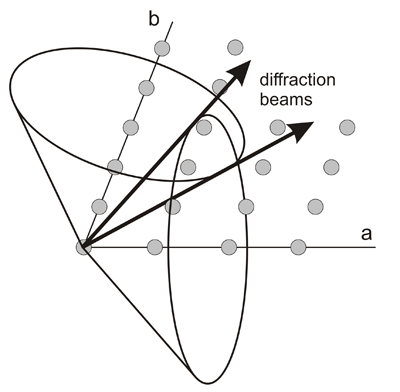
\includegraphics[width= 4 cm] {laue.jpg}
\end{figure}

\vskip 2 mm

\subsection {Derivation of Laue's equation of diffraction for x-rays}
Let $P_1$ and $P_2$ be two such lattice points separated by a vector $\vec{r}$. 
Suppose a parallel beam of x-rays is incident on $P_1P_2$ along the direction of unit vector $\hat{i}$.
The scattered beam is also parallel and let it be in any arbitrary direction given by unit vector $\hat{s}$.

Now on drawing $P_1A$ perpendicular to the incident wave's direction and $P_2B$ perpendicular to the scattered wave's direction, then $P_1A$ is the incident and $P_2B$ is the scattered wave font.

The path difference between the two scattered waves - one scattered from $P_2$, and the other scattered from $P_1$ is given by
$$ P_2A - P_1B = \vec{r}.\hat{i} - \vec{r}.\hat{s} = \vec{r}.(\hat{i}-\hat{s}) = \vec{r}.\vec{S}                              \qquad\qquad\qquad -(1)$$
where, $\vec{S} = (\hat{i}-\hat{s})$ is a vector in the direction of the normal to the reflecting surface.
[The set of all wave vectors $\vec{S}$ that yields plane wave with the periodicity of a given Bravais lattice is known as Reciprocal lattice]

If $\theta$ is the angle that the incident beam makes with the reflecting plane, then the angle that the scattered or reflected beam makes with the reflecting plane is also equal to $\theta$ and the angle between the unit vectors $\hat{i}$ and $\hat{s}$.
$$ |\vec{S}| = 2\sin \theta                 \qquad\qquad\qquad\qquad\qquad\qquad -(2)$$

The phase difference between the waves scattered at the lattice points$P_1$ and $P_2$ is given by $$ \phi = \frac{2\pi}{\lambda} (\vec{r}.\vec{S}) \qquad\qquad\qquad\qquad\qquad\qquad -(3)$$

The intensity of the diffracted beam is a maximum in the direction in which $\phi$ is an integral multiple of $2\pi$.

\begin{figure}[h!]
  \centering 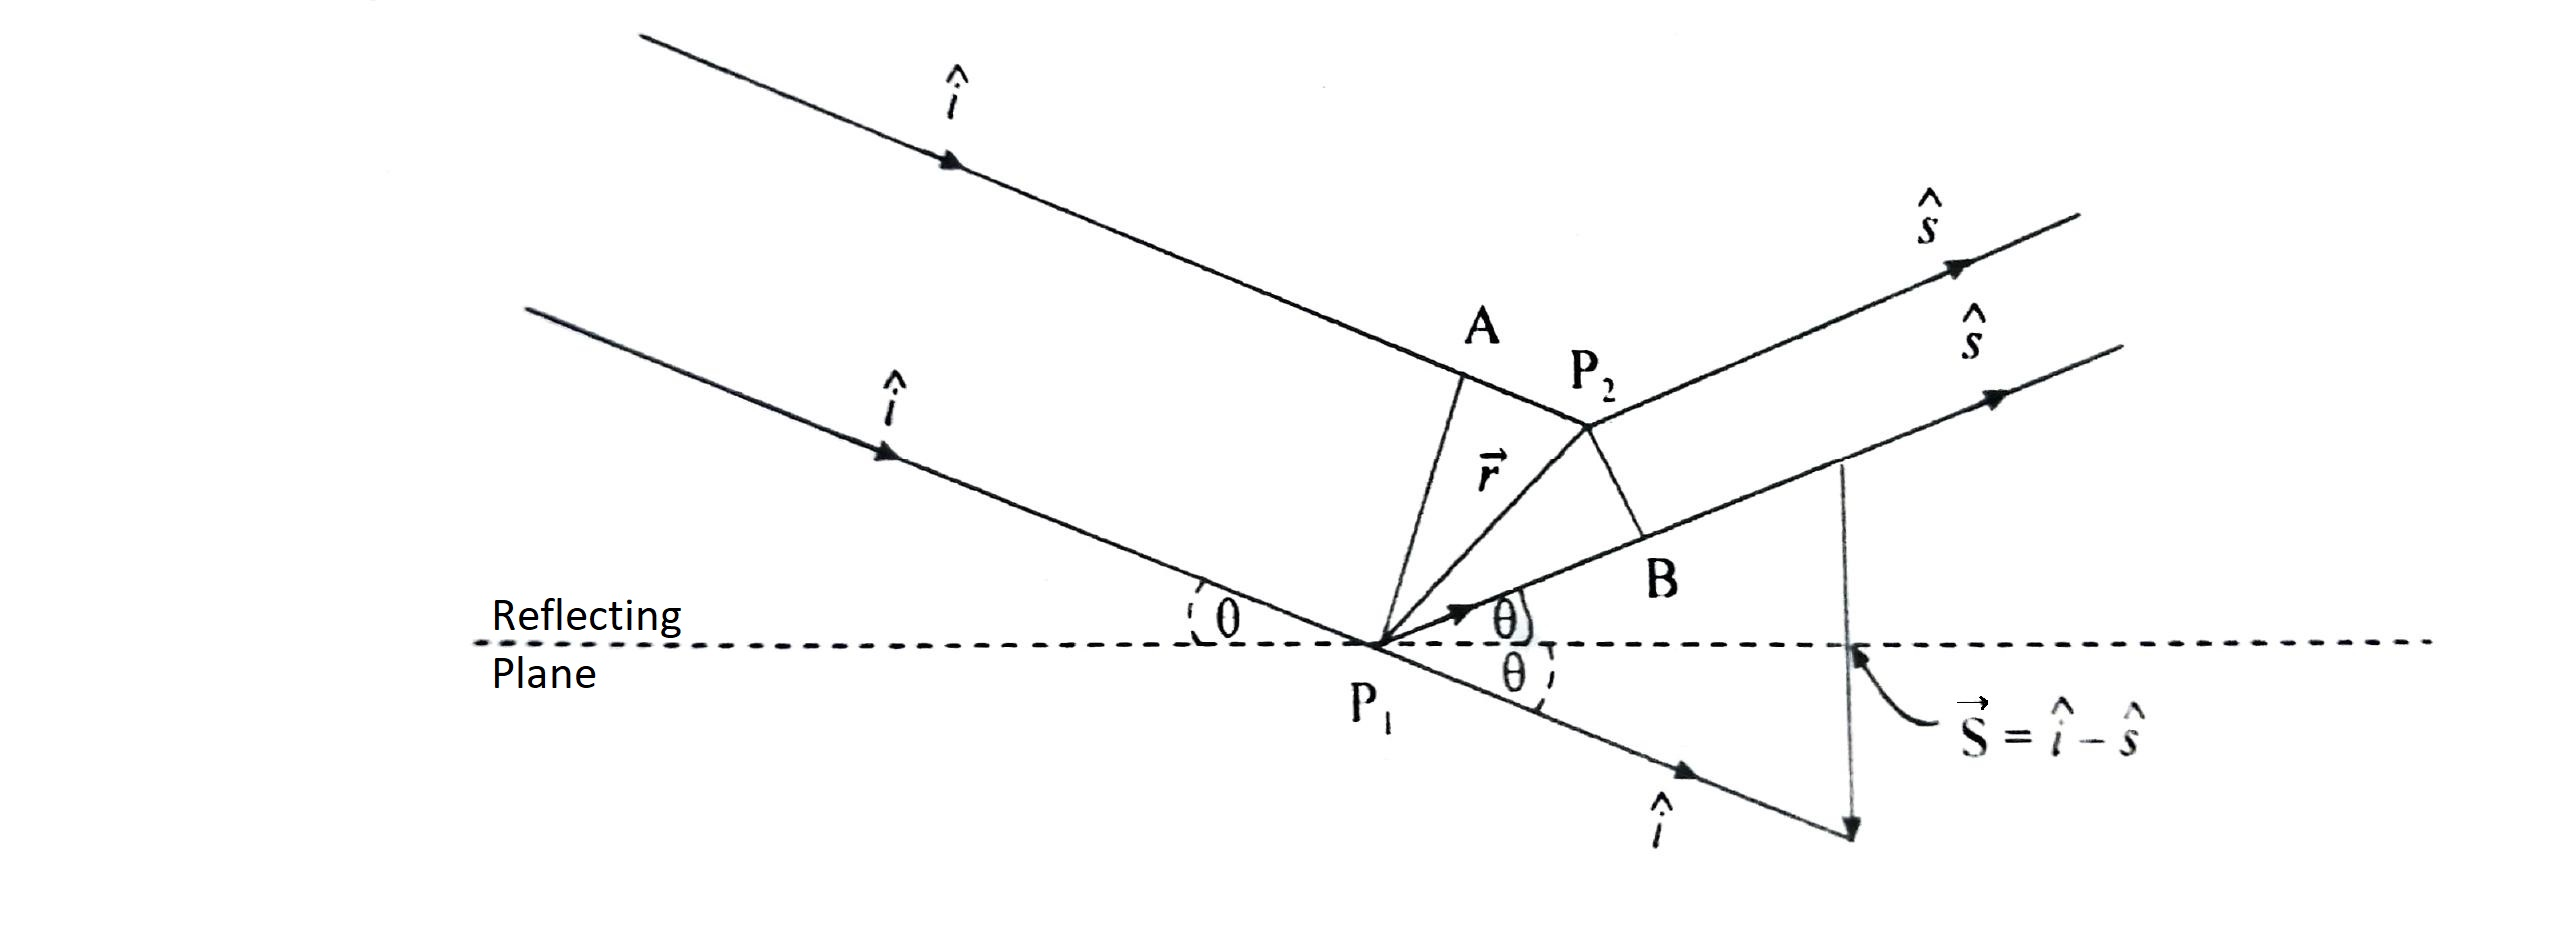
\includegraphics[width= 18cm] {la.jpg}
\end{figure}

If $\vec{a},\vec{b},\vec{c}$ are the primitive lattice vectors of the point $P_2$ w.r.t. the point $P_1$, then $$\vec{r}=\vec{a}+\vec{b}+\vec{c} \qquad\qquad\qquad\qquad\qquad\qquad -(4)$$

And the above conditions can be put in the form of three seperate conditions,i.e.,
$$ \phi_a = \frac{2\pi}{\lambda} (\vec{a}.\vec{S}) \qquad\qquad\qquad\qquad\qquad -(5)$$
$$ \phi_b = \frac{2\pi}{\lambda} (\vec{b}.\vec{S}) \qquad\qquad\qquad\qquad\qquad -(6)$$
$$ \phi_c = \frac{2\pi}{\lambda} (\vec{c}.\vec{S}) \qquad\qquad\qquad\qquad\qquad -(7)$$
where $h,k,l$ are the integers and $\phi_a,\phi_b,\phi_c$ are phase differences between the waves scattered from the two ends of the primitive lattice vectors $\vec{a},\vec{b},\vec{c}$ respectively.

Therefore, we can now re-write eqn.(5),(6),(7) and get :-
$$ \vec{a}.\vec{S} = h\lambda \qquad\qquad\qquad\qquad\qquad\qquad\qquad -(8)$$
$$ \vec{b}.\vec{S} = k\lambda \qquad\qquad\qquad\qquad\qquad\qquad\qquad -(9)$$
$$ \vec{c}.\vec{S} = l\lambda \qquad\qquad\qquad\qquad\qquad\qquad\qquad -(10)$$

If $\alpha,\beta,\gamma$ be the angles between the normal to the reflecting plane and $\vec{a},\vec{b},\vec{c}$ axes respectively, then
$$ \vec{a}.\vec{S} = |\vec{a}||\vec{S}|\cos \alpha = 2a\sin\theta\cos\alpha \qquad\qquad -(11)$$
$$ \vec{b}.\vec{S} = |\vec{b}||\vec{S}|\cos \beta = 2b\sin\theta\cos\beta   \qquad\qquad -(12)$$
$$ \vec{c}.\vec{S} = |\vec{c}||\vec{S}|\cos \gamma = 2c\sin\theta\cos\gamma \qquad\qquad -(13)$$

Now from (8),(9),(10) and (11),(12),(13), we get :
$$ 2a\sin\theta\cos\alpha = h\lambda   \qquad\qquad\qquad\qquad\qquad\qquad -(14)$$
$$ 2b\sin\theta\cos\beta  = k\lambda   \qquad\qquad\qquad\qquad\qquad\qquad -(15)$$
$$ 2c\sin\theta\cos\gamma = l\lambda   \qquad\qquad\qquad\qquad\qquad\qquad -(16)$$
These above equations are the Laue's equations for X-ray diffraction.


\subsection{Derivation of Bragg's relation from Laue's equations.}
Now if we consider $\theta$ as the given direction of Bragg diffraction for a wavelength $\lambda$, then the direction cosines of $\vec{S}$ the scattering normal from equations (14),(15),(16) are thus given by
$$ \cos \alpha = \frac{\lambda}{2\sin\theta}\frac{h}{a} \qquad\qquad\qquad\qquad\qquad\qquad -(17)$$
$$ \cos \beta = \frac{\lambda}{2\sin\theta}\frac{k}{b} \qquad\qquad\qquad\qquad\qquad\qquad -(18)$$
$$ \cos \gamma = \frac{\lambda}{2\sin\theta}\frac{l}{c} \qquad\qquad\qquad\qquad\qquad\qquad -(19)$$
$i.e.,$the direction cosines are respectively proportional to $\frac{h}{a},\frac{k}{b},\frac{l}{c}$.

Now the adjacent lattice planes whose Miller indices are $(h,k,l)$ intersect the $\vec{a},\vec{b},\vec{c}$ axes at the intervals $\large{\frac{a}{h},\frac{b}{k},\frac{c}{l}}$.

Thus we find that the scattering normal $\vec{S}$ is identical to the normal to $(hkl)$ planes.
Now the $(hkl)$ planes may be regarded as the reflecting planes of Bragg's diffraction.

If $d(hkl)$ is the spacing between two adjacent planes of a set $(hkl)$, then
$$(hkl)=\frac{a}{h}\cos\alpha=\frac{b}{k}\cos\beta=\frac{c}{l}\cos\gamma \qquad\qquad\qquad\qquad\qquad\qquad -(20)$$

Now according to Laue's equations
$$\frac{a}{h}\cos\alpha=\frac{b}{k}\cos\beta=\frac{c}{l}\cos\gamma=\frac{\lambda}{2\sin\theta} \qquad\qquad\qquad\qquad\qquad\qquad -(21)$$
which can be put in the form from $eqn.(20),(21)$, we get
$$ d(hkl)=\frac{\lambda}{2\sin\theta}$$
$$or, \qquad\qquad\qquad\qquad\qquad 2d(hkl) \sin\theta=\lambda \qquad\qquad\qquad\qquad-(22)$$

The integers $h,k,l$ of Laue's equation are not necessarily identical with Miller indices of an actual crystal plane but these integers may contain a common factor , let us say $n$, while in the indices the common factor has been eliminated.

So here on introducing the common factor $n$, we get $$ 2d \sin \theta = n\lambda  \qquad\qquad\qquad\qquad\qquad\qquad\qquad\qquad\qquad\qquad -(23)$$ where ${d}$ is the spacing between adjacent planes with Miller indices $\large{\frac{h}{n},\frac{k}{n},\frac{l}{n}}$ 
and $eqn.(23)$ is the Bragg's relation for an angle $\theta$ between the incident beam and the reflecting plane.
 
[ Miller indices of a lattice plane are the coordinates of the shortest reciprocal lattice vector normal to that plane, w.r.t. a specified set of primitive reciprocal lattice vectors. Thus a plane with Miller indices $h,k,l$ is normal to the reciprocal lattice vector $h\vec{a}+k\vec{b}+l\vec{c} $]

\vskip 18 mm
\section {Laue's method :}
In this method a single crystal is held stationary in a beam of X-rays of continuous wavelength. Laue's X-ray camera consists of a source producing X-rays of a continuous wavelength over a wide range (perhaps from 0.2$\mathring{A}$ to 2$\mathring{A}$), a pin hole collimator which produces a very fine narrow beam, a single crystal specimen which is not more than a one mm in size held stationary in a stand and two flat films on which the diffracting patterns are recorded.

\begin{figure}[h!]
  \centering 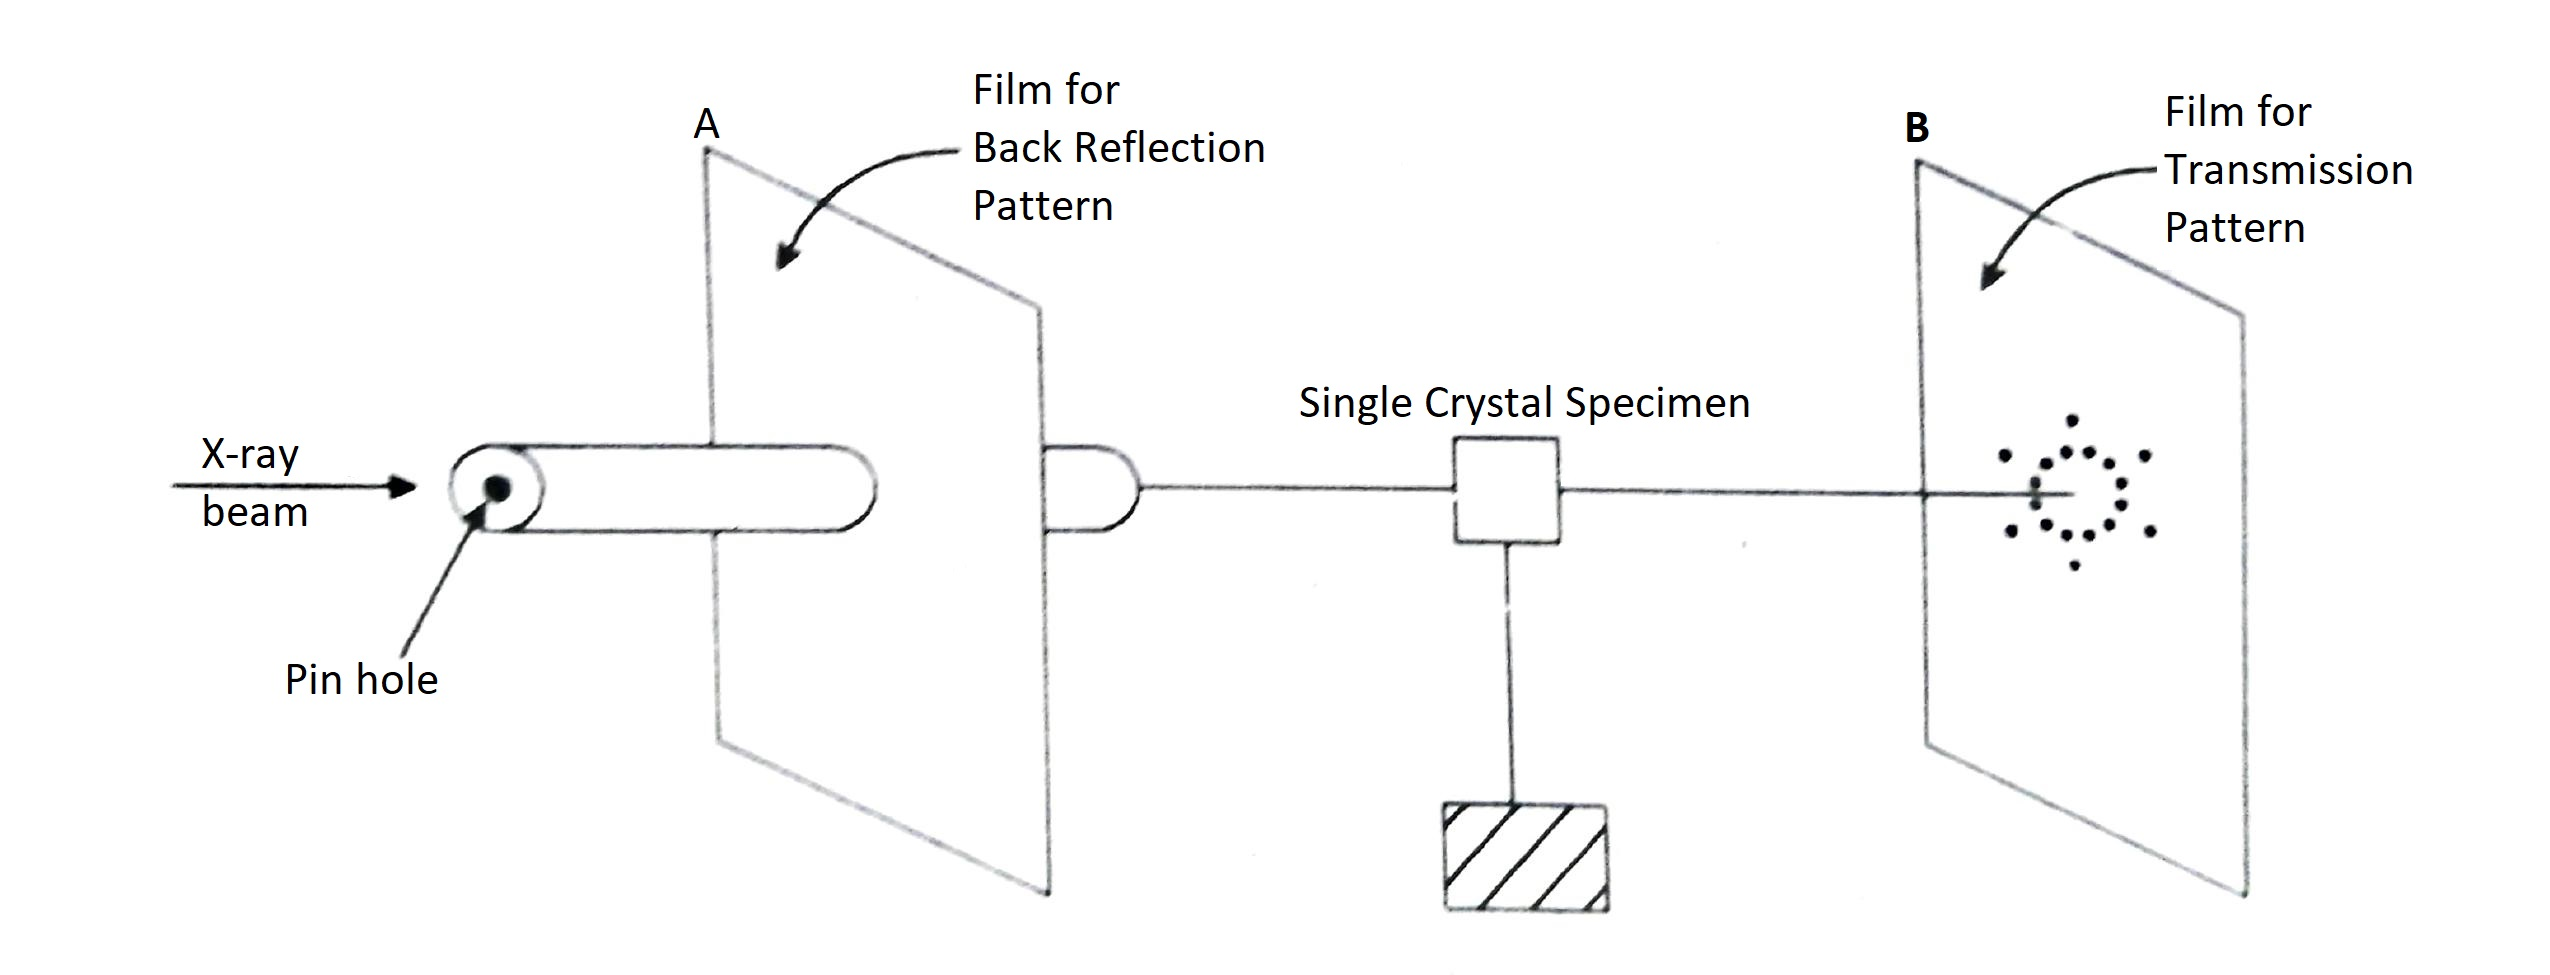
\includegraphics[width= 16cm] {lau.jpg}
\end{figure}

 The film A records the back reflection pattern and the film B records the transmission pattern.
The crystal selects and produces diffraction corresponding to discrete values of $\lambda$ for which planes of spacing ${d}$ exist and angle of incidence $\theta$ satisfies Bragg's relation. The diffraction pattern consists of a series of spots known as Laue spots showing the symmetry of the crystal. 



For example : If a crystal with four-fold axis of symmetry is oriented with the axis parallel to the beam, the Laue pattern will show four-fold symmetry. The symmetry helps to determine the shape of the unit cell. This feature makes it specially useful for checking the orientation of crystals in solid state experiments.

\vskip 20 mm

\subsection{Usefulness of the method in Solid State Physics}
\begin {enumerate}
\item It is suitable for the rapid determination of crystal orientation and symmetry. 
\begin{figure}[h!]
  \centering 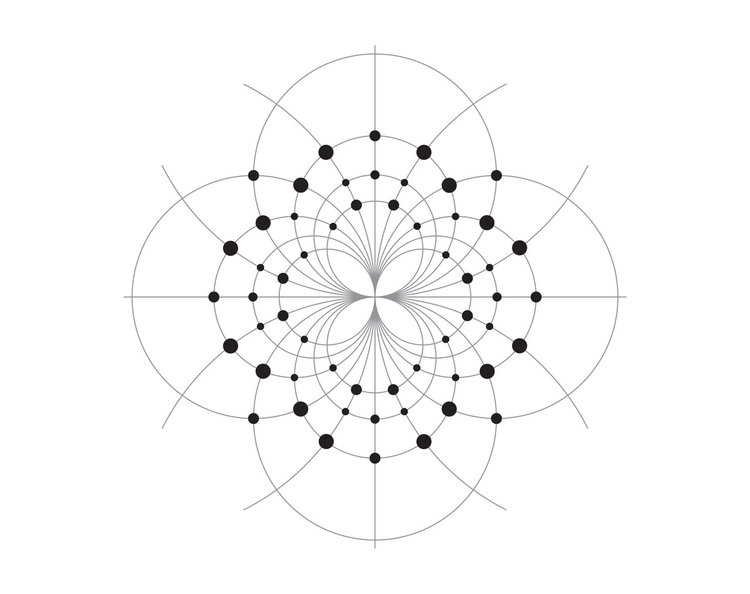
\includegraphics[width= 14cm] {fourfold.jpg}
\end{figure}

From the above stated example we can conclude that the symmetry of the pattern helps to determine the shape of the unit cell.
\item An imperfect or strained crystal has atomic planes which are not exactly plane but are slightly curved. Therefore, instead of sharp diffraction spots we get streaks in Laue's pattern. The formation of streaks on Laue's photographs is known as $\textbf{asterism}$.
This method is thus used for studying the extent of crystalline imperfection under mechanical and thermal treatment.
\end{enumerate}
\subsection{Arising Problem of the method in Solid State Physics}
\begin {enumerate}
\item This method is not suitable for determining crystal structure. It is because out of the continuous range of wavelengths, several wavelenghts are reflected in different orders from a single plane and have different order reflections may overlap on a single spot.
\end{enumerate}
\vskip 40 mm
\section{Some Experimental Data}
\begin{enumerate}
\item Sodium Chloride (NaCl) Single Crystal

Laue Pattern obtained with a sodium chloride single crystal sample (100) oriented. Exposure time of 2 h. Copper anode x-ray tube, $Va = 30 KV$, $Ia = 60 \mu A$. The symmetry for rotation of $2\pi / 4 $characteristic of the cubic structure is evident.
The image below shows the Laue diagram of a NaCl (100) single crystal with a face-center cubic crystal lattice (fcc). If the diffraction pattern is rotated by 90° around the direction of the primary beam, it is again brought to coincidence. Since the primary beam impinges perpendicularly on the (100)-plane of the NaCl crystal, the crystal direction [100] is a fourfold axis of symmetry. The intensity of the reflections depends on the reflecting crystal surface as well as on the spectral intensity distribution of the X-rays.
\begin{figure}[h!]
  \centering 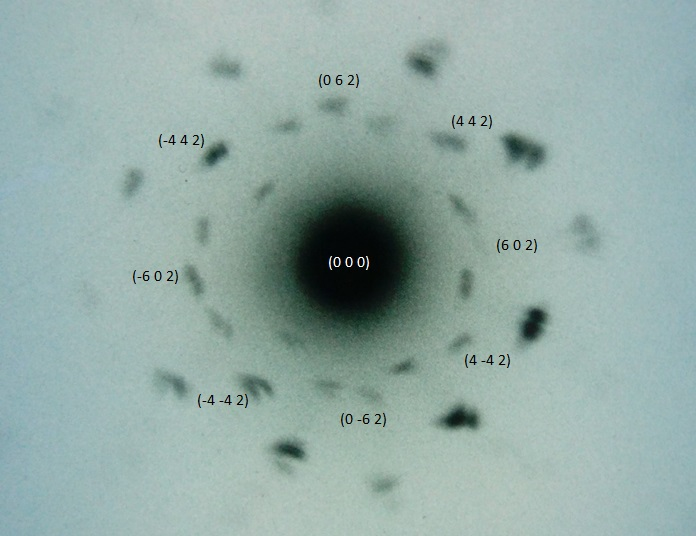
\includegraphics[width= 10cm] {NaCl.jpg}
\end{figure}
\vskip 1 mm
\item Silicon Single Crystal

Laue Pattern obtained with a single crystal silicon sample (100) oriented. Exposure time of 1 h. Copper anode x-ray tube, $Va = 30 KV, Ia = 60 \mu A$. The symmetry for rotation of $2\pi / 4$ characteristic of the cubic structure is evident
\begin{figure}[h!]
  \centering 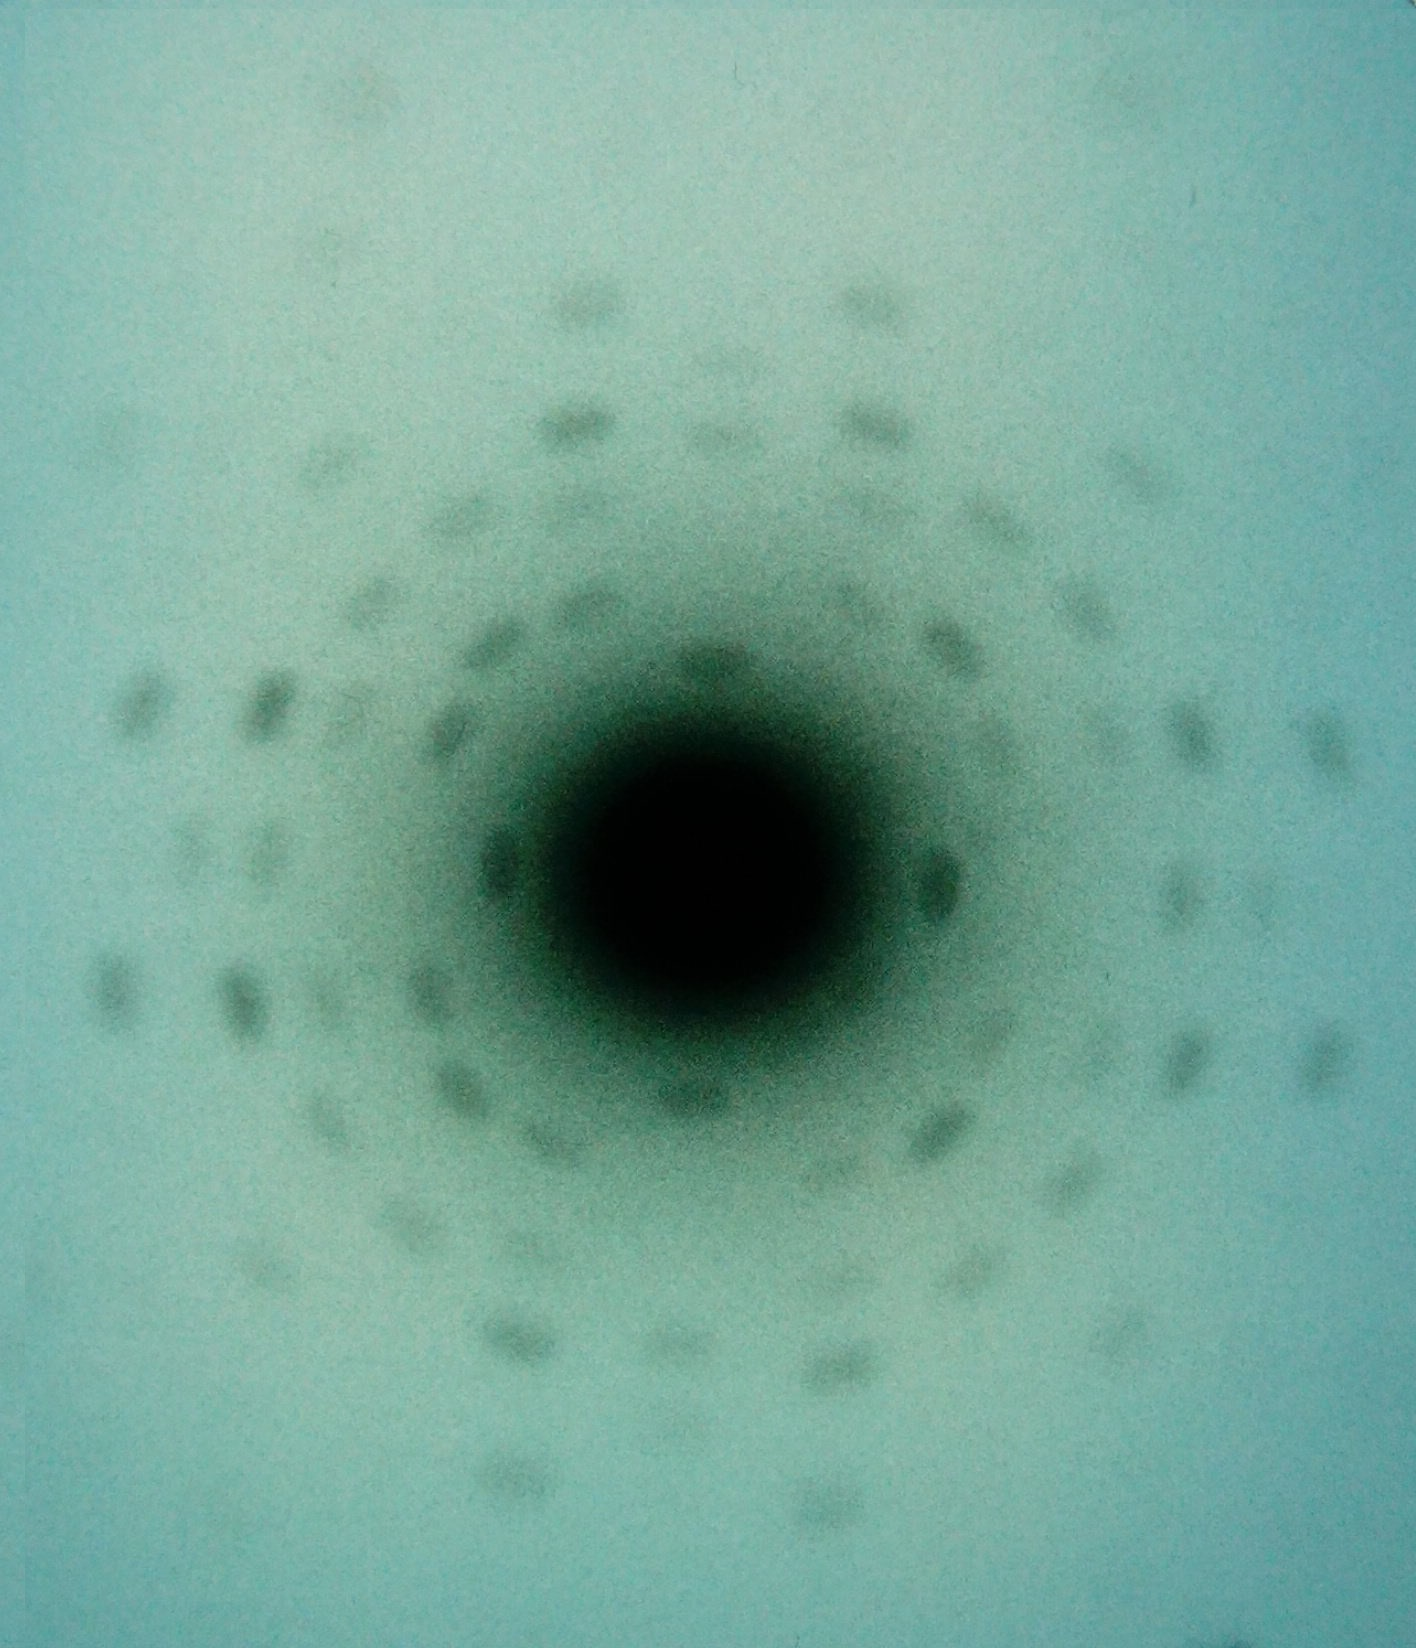
\includegraphics[width= 5cm] {Silicon.jpg}
\end{figure}

\vskip 3 mm

\item Fluorite Single Crystal

Laue Pattern obtained with a single crystal Fluorite sample (111) oriented. Exposure time of 2 h. Copper anode x-ray tube,$ Va = 30 KV, Ia = 60 \mu A$. The threefold symmetry for rotation of $2\pi / 3$ characteristic of the cubic structure oriented on the diagonal of cube is evident
\begin{figure}[h!]
  \centering 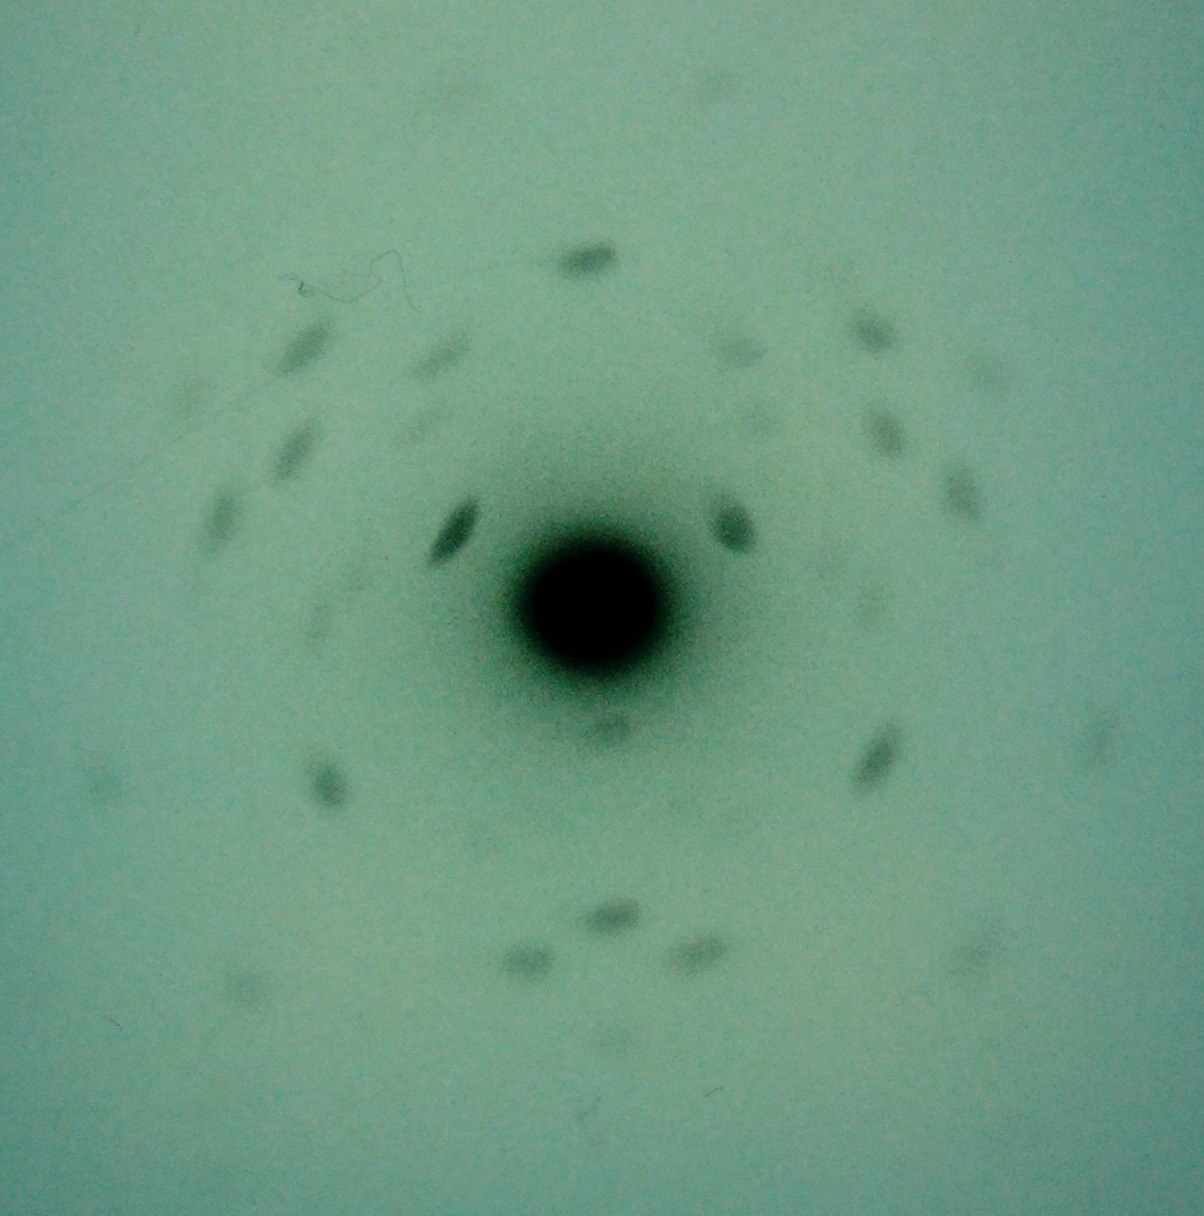
\includegraphics[width= 8cm] {fluorite.jpg}
\end{figure}
\vskip 10 mm
\item Quartz Single Crystal

Laue Pattern obtained with a single crystal Quartz sample (100) oriented. Exposure time of 2 h. Copper anode x-ray tube, $Va = 30 KV, Ia = 60 \mu A.$
\begin{figure}[h!]
  \centering 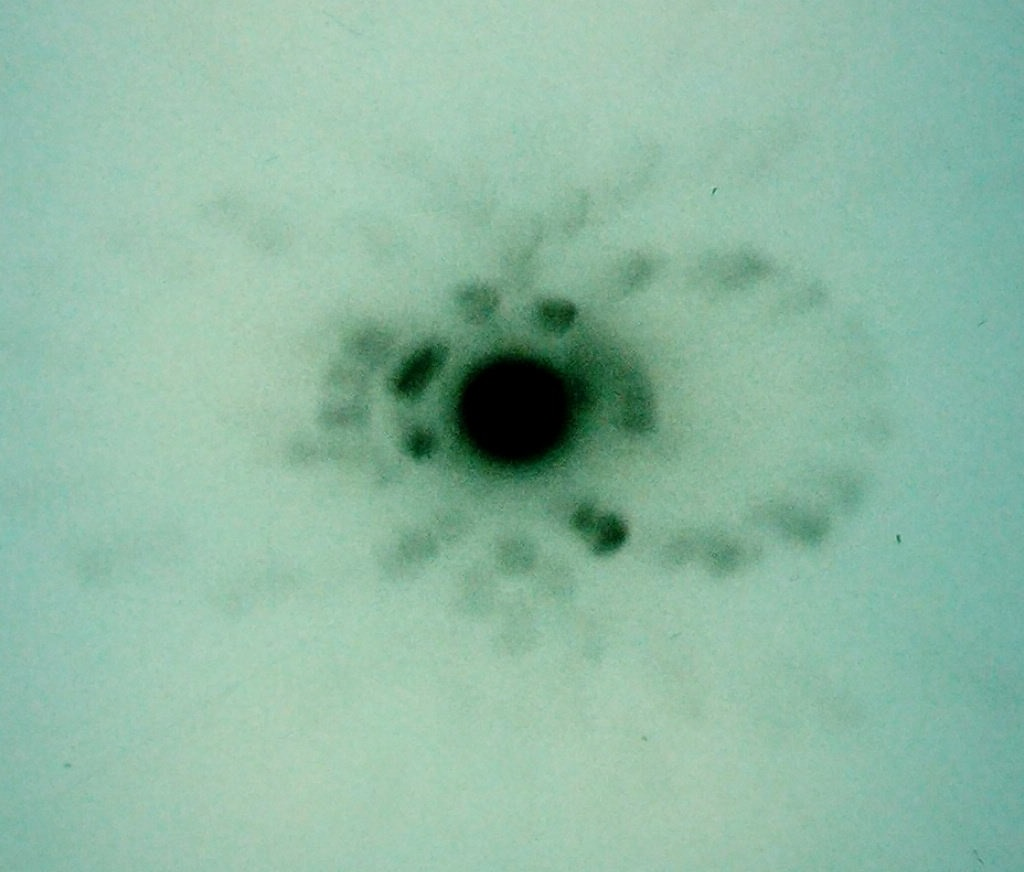
\includegraphics[width= 10cm] {quartz.jpg}
\end{figure}

\vskip 10 mm

\item Gypsum Single Crystal

Laue Pattern obtained with a single crystal Gypsum sample (020) oriented. Exposure time of 2 h. Copper anode x-ray tube,$ Va = 30 KV, Ia = 60 \mu A.$
\begin{figure}[h!]
  \centering 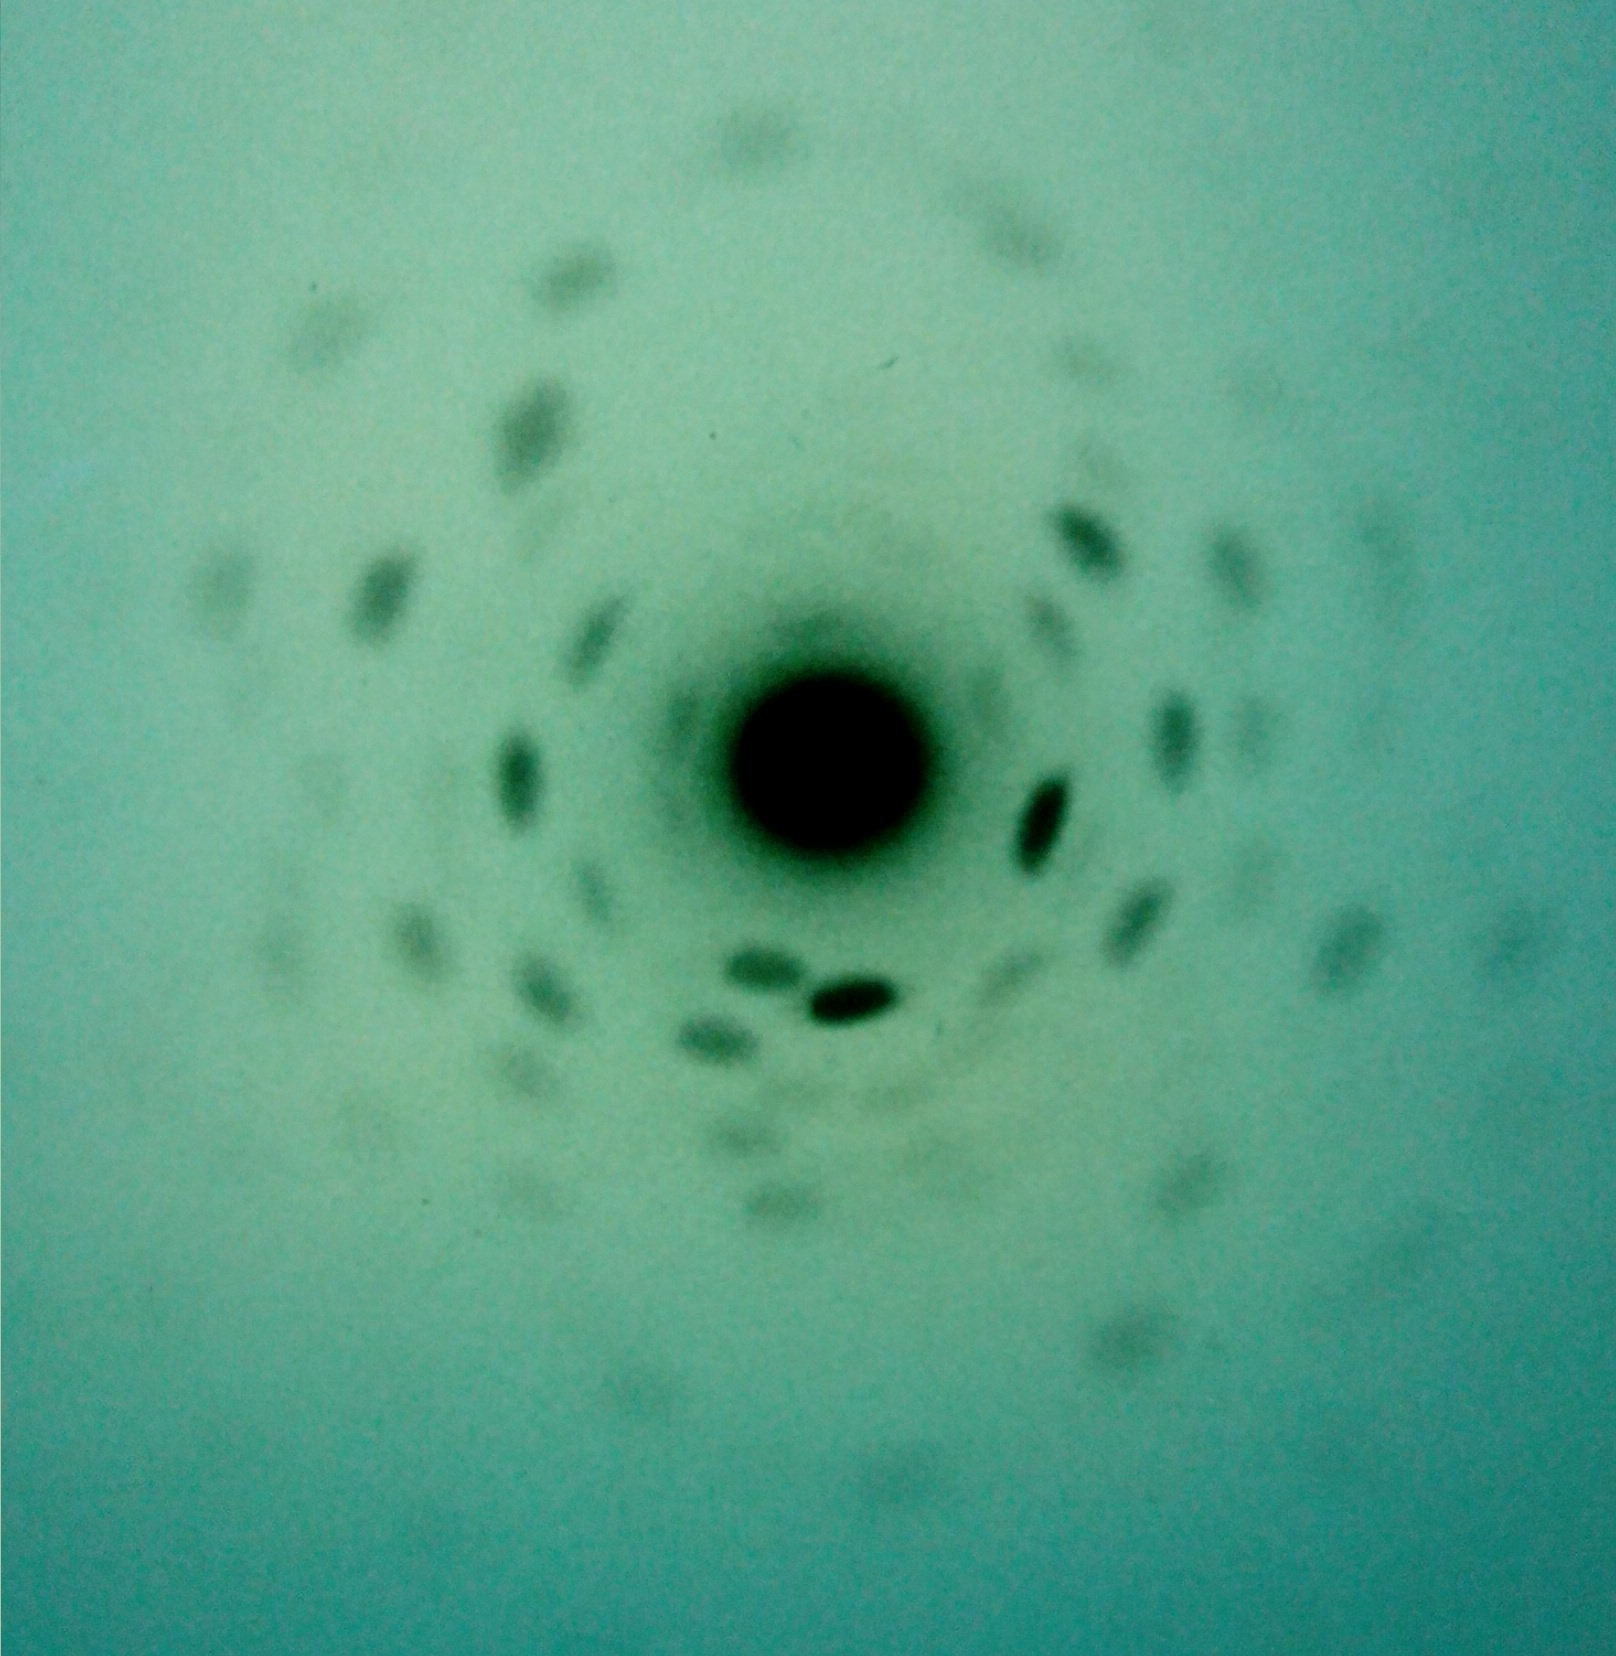
\includegraphics[width= 10cm] {gypsum.jpg}
\end{figure}
\vskip 8 mm
\item Sphalerite (Zinc Blende)

Laue Pattern obtained with a single crystal Sphalerite sample (100) oriented. Exposure time of 1 h. Copper anode x-ray tube,$ Va = 30 KV, Ia = 60 \mu A$. Sphalerite ((Zn, Fe)S) is a mineral that is the chief ore of zinc. It consists largely of zinc sulfide in crystalline. Evident the four-fold simmetry, feature of cubic crystal cell.
\begin{figure}[h!]
  \centering 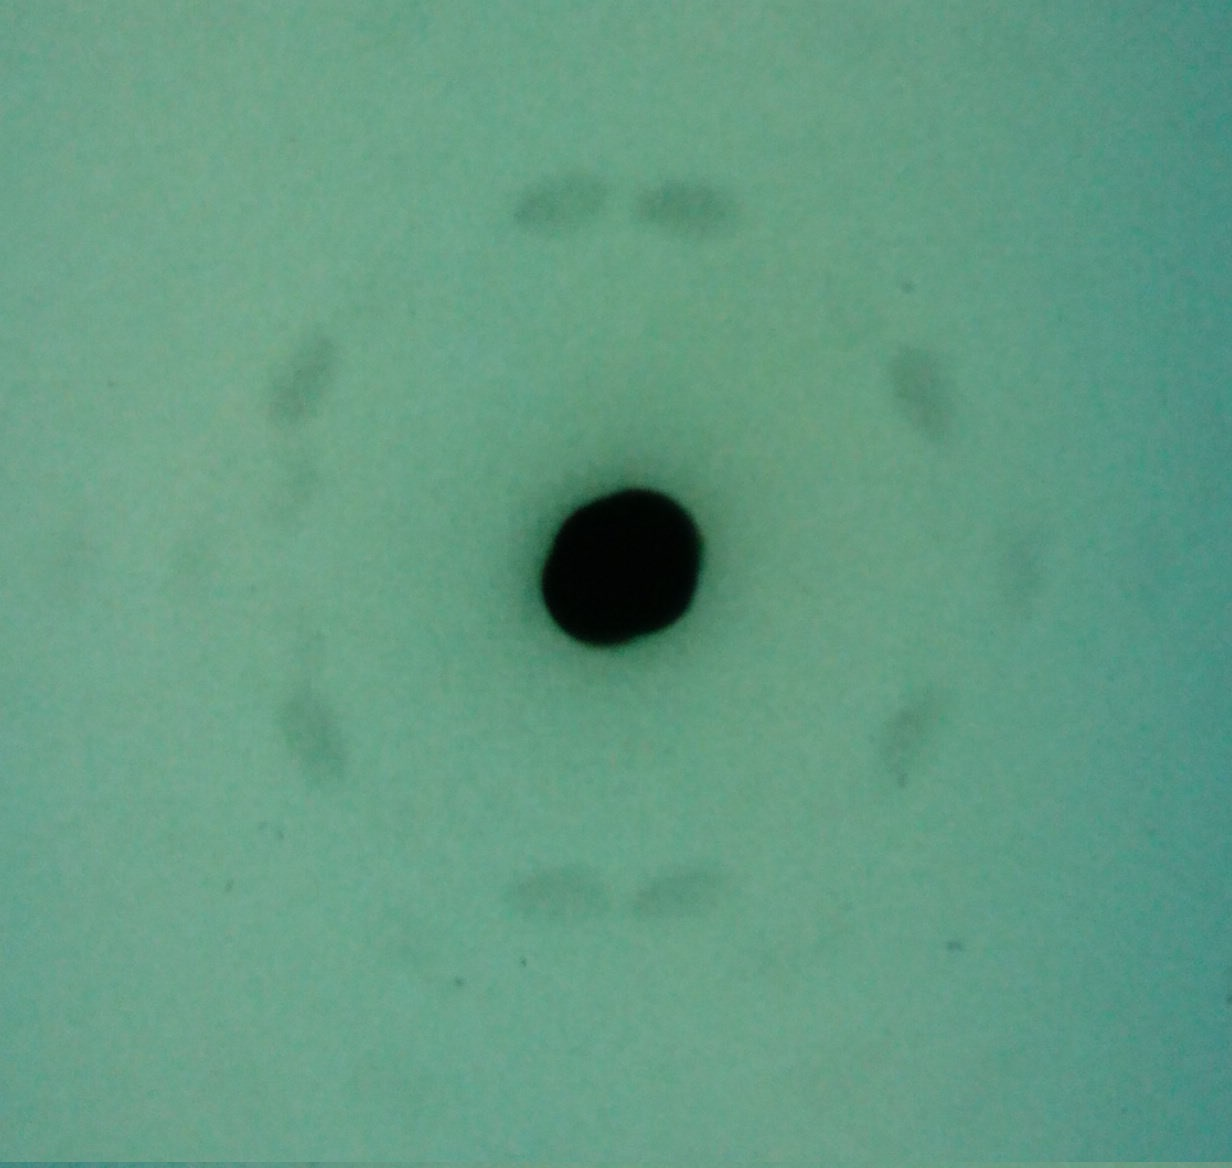
\includegraphics[width= 7cm] {zinc.jpg}
\end{figure}
\end{enumerate}

\vskip 10 mm
\begin{thebibliography}{9}
\bibitem{Kittel}
  Charles Kittel ,
  \textit {Kittel's Introduction to Solid State Physics}
  Chapter 2,
  Wiley,
  2019 
 \bibitem{Ashcroft/Mermin}
   N. David Mermin, Neil W. Ashcroft ,
   \textit {Solid State Physics},
   Chapter 6,
   Cengage,
   2003
  \bibitem{Ali}
  OMAR ALI ,
 \textit {Elementary Solid State Physics, 1e},
 Chapter 2,
  Pearson ,
  2002
 \bibitem{Internet}
 \textit{https://physicsopenlab.org/2018/01/18/laue-diffraction/}
 External Resources
\end{thebibliography}  
\end{document}
